\begin{document}

\def\title{Homework 8}
% \config{hwnum}{2}
% \config{homework-due}{02/0/2019 23:59}
% \config{grades-due}{02/XX/2019 23:59}

\newcommand{\qitem}{\qpart\item}

\renewcommand{\labelenumi}{(\alph{enumi})} % change default enum format to (a)
\renewcommand{\theenumi}{(\alph{enumi})} % fix reference format accordingly.
\renewcommand{\labelenumii}{\roman{enumii}.} % second level labels.
\renewcommand{\theenumii}{\roman{enumii}.}

\maketitle
% \vspace{0.5em}
% {\textbf{Due date:} 2/8/19, at 23:59. Please \LaTeX of handwrite your homework solution and submit an electronic version on Gradescope.}

% {\textbf{Self-grades due date:} 2/XX/19, at 23:59.}

% {\parindent 0pt
% \begin{tabular}[t]{l}
% EECS 127 / EE 227AT \\
% G. Ranade, A. Bayen
% \end{tabular}  \hfill 2/1/19\vskip 0.2in }

% \parindent 0pt
% \parskip 8pt

% \begin{center}
% \large\bf Homework Assignment \#2
% \end{center}

% \bigskip

\noindent
{\bf Release date:}  10/24/19 \\
{\bf Due date:}  10/31/19, 23:00 (11 pm). Please \LaTeX{} or handwrite your homework solution and submit an electronic version.

\textbf{Submission Format} \\
Your homework submission should consist of a single PDF file that contains all of your answers (any handwritten answers should be scanned) as well as your IPython notebook saved as a PDF.
			
If you do not attach a PDF ``printout'' of your IPython notebook, you will not receive credit for problems that involve coding. Make sure that your results and your plots are visible. Assign the IPython printout to the correct problem(s) on Gradescope.


\begin{qunlist}
\qns{LASSO vs. Ridge}\rm

Say that we have the data set $\{ (x^{(i)}, y^{(i)}) \}_{i=1,\dots, n}$ of features $x^{(i)} \in \Real{d}$ and values $y^{(i)} \in \Real{}$. Define $X = \begin{bmatrix} {x^{(1)}} & \dots & {x^{(n)}} \end{bmatrix}\tran$ and $y = \begin{bmatrix} y^{(1)} & \dots & y^{(n)} \end{bmatrix}\tran$.
For the sake of simplicity, assume that the data
has been centered and whitened so that
each feature has mean $0$ and variance $1$ and the features are uncorrelated, i.e. $X\tran X = n I$.

Consider the linear least squares regression with regularization in the $\ell_1$-norm, also known as LASSO:
\[w^* = \arg \min_{w \in \Real{d}} \; \|X w - y\|_2^2 + \lam \|w\|_1\]

This problem will compare $\ell_1$-regularization with $\ell_2$-regularization (ridge regression) to understand their similarities and differences. We will do this by looking at the elements of $w^*$ in the solution to each problem.

\begin{enumerate}
\qitem {[Few lines of justification]} First, decompose this optimization problem into $d$ univariate optimization problems over each element of $w$. Let $X = \begin{bmatrix}x_1 & \ldots & x_d\end{bmatrix}$.

\newline
\sol{\item $g(x_1,x_2) = \dfrac{x_1^2}{4} + \dfrac{x_2^2}{9}$


}
\newline

\qitem {[Short justification, 1-2 lines]} If $w_i^* > 0$, then what is the value of $w_i^*$? What is the condition on $y\top x_i$ for this to be possible?

\newline
\sol{\item Show that the following inequalities hold for any vector $x \in \Real{n}$:
\[
% \|x\|_\infty \le \|x\|_1 \le n \|x\|_\infty \\
% \|x\|_2 \le \|x\|_1 \le \sqrt{n} \|x\|_2 \\
% \|x\|_\infty \le \|x\|_2 \le\sqrt{n}\|x\|_\infty \\
\frac{1}{\sqrt{n}}\|x\|_2 \leq \|x\|_\infty \leq  \|x\|_2 \leq \|x\|_1 \leq \sqrt{n} \|x\|_2 \le n\|x\|_\infty.
\]

\textit{Hint:} For $\|x\|_1\leq \sqrt{n}\|x\|_2$, how might you express $\|x\|_1$ as the dot product of two vectors? Can you then use the Cauchy-Schwarz inequality to bound this dot product?}
\newline

\qitem {[Short justification, 1-2 lines]} If $w_i^* < 0$, then what is the value of $w_i^*$? What is the condition on $y^\top x_i$ for this to be possible?

\newline
\sol{\item $g(x) = \sin(x_1^2) \log (x_3 - x_2)$ where $x_i$ are scalars and $x_3 - x_2 > 0$.}
\newline

\qitem {[Short justification, 1-2 lines]} What can we conclude about $w_i^*$ if $|y^\top x_i| \leq \dfrac{\lambda}{2}$? How does the value of $\lambda$ impact the individual entries $w_i^*$?

\newline
\sol{\item
\[
g(x) = \begin{bmatrix}
x_1^2/x_2 \\
\log(x_3) \sin(x_1/x_3)
\end{bmatrix}
\]}
\newline

\qitem {[Few lines of justification]} Now consider the case of ridge regression, which uses the the $\ell_2$ regularization $\lam \|w\|_2^2$.
\[w^* = \arg \min_{w \in \Real{d}} \; \|X w - y\|_2^2 + \lam \|w\|_2^2\]
What is the new condition for $w_i^*$ to be $0$? How does this differ from the condition obtained in part (d)? What does this suggest about LASSO?

\newline
\sol{\input{ridge_lasso_sol/5.tex}}
\newline

\end{enumerate}

\newpage
\qns{Image Compression}
\newline
Most of the work for this question will be done in \verb|image_compression.ipynb|. The questions below are to help you write out the math that you will implement in code. 

\begin{enumerate}
    \item {[Single line expression]} If $\mathbf{A}\in \R^{m\times n}$ $= U\Sigma V^T$, what is a rank $k$ approximation of $\mathbf{A}$ in terms of the columns and rows of $U$,$\Sigma$,$V^T$. Explicitly express the dimensions of your matrices.
    \newline
    \sol{\item $g(x_1,x_2) = \dfrac{x_1^2}{4} + \dfrac{x_2^2}{9}$


}
    \newline
    \item {[Single line expression]} We aim to learn a sparse representation $\hat{y}\in\R^{m\times n}$ of some data $y\in\R^{m\times{n}}$. Formulate this as a LASSO problem (using the Frobenius and L1 norms).
    \newline
    \sol{\item Show that the following inequalities hold for any vector $x \in \Real{n}$:
\[
% \|x\|_\infty \le \|x\|_1 \le n \|x\|_\infty \\
% \|x\|_2 \le \|x\|_1 \le \sqrt{n} \|x\|_2 \\
% \|x\|_\infty \le \|x\|_2 \le\sqrt{n}\|x\|_\infty \\
\frac{1}{\sqrt{n}}\|x\|_2 \leq \|x\|_\infty \leq  \|x\|_2 \leq \|x\|_1 \leq \sqrt{n} \|x\|_2 \le n\|x\|_\infty.
\]

\textit{Hint:} For $\|x\|_1\leq \sqrt{n}\|x\|_2$, how might you express $\|x\|_1$ as the dot product of two vectors? Can you then use the Cauchy-Schwarz inequality to bound this dot product?}
    \newline
    \item Follow the instructions in \verb|image_compression.ipynb|
\end{enumerate}
\newpage
\qns{Image Restoration}
\newline
\newline
Finally! You did it!! After years of trying you finally got the perfect shot of the campanile. You were so excited you decided you should post it on Instagram. But first, you wanted to share it with your friends. You called them over and showed it to them. Your friends are from Stanford. They thought it would be cool to play a trick on you, so they edited your picture by adding the text `` I wish I was at Stanford though! :( ". 

\begin{figure}[h]
\centering
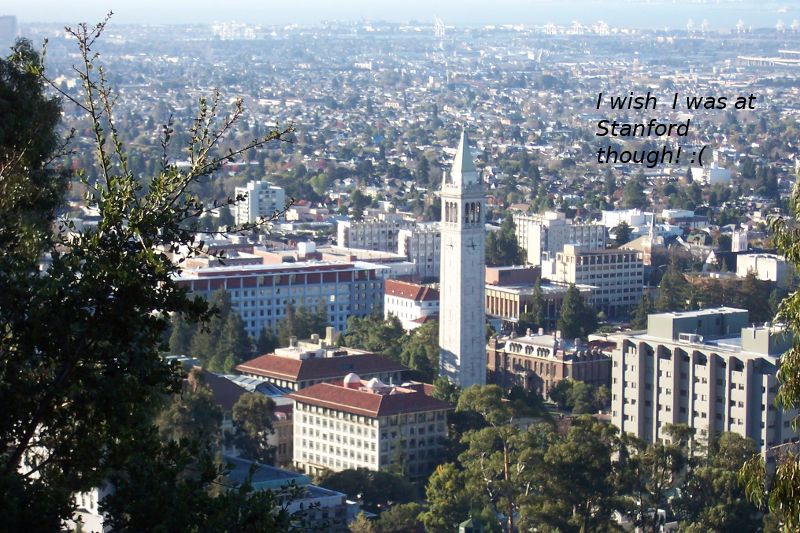
\includegraphics[scale=2.00]{figures/campanile_img_corrupted.jpg}
\caption{Your perfect shot corrupted by your Stanford friends :(}
\end{figure}
You see this in the morning, and realize you had no backup of your photo. While the prank was in good fun, you would like to get your original image back. So, you apply your Berkeley smarts in order to recreate the original image. You will be completing an exercise to try to restore the image your friends corrupted.
\newline
\newline
First, we will need to understand the representation an image (grayscale) stored in memory as a discrete sampling of a function over a continuous domain. One can think of an image as a function $f(x,y)\colon \Omega \subset  \mathbb{R}^{2}\to \mathbb{R}_{+}$.  The range represents the color intensity at each point in the image.
\newline
\newline
To make the definition more concrete, we choose $\Omega = \{(x,y): 1 \leq x \leq W+1,1 \leq y \leq H+1 \}$. Also in practice, the range of the function $f$ may be restricted to the set $[0,255]$, with $0$ being black, $255$ being white, and the numbers in between being various shades of gray going from dark to light. 
\newline
\newline
When we store the image in memory, we sample this function at discrete points and store these samples (typically as a matrix). Given a fixed matrix with $W$ rows and $H$ columns. We may denote the sampled version of the function as: $F(i,j), \hspace{5pt} i \in {1,2, \hdots , W}, \hspace{5pt} j\in {1,2, \hdots , H} $. 
\begin{enumerate}
    \item {[Few lines of justification]}
     To sample an image and ensure that we cover the domain, we may partition the domain into equal sized intervals and sample a point from each interval. One way to do this is to partition the interval of $x$ values over the domain into intervals of width $1$ and to partition the interval of $y$ values of width $1$. We may then sample points on the left boundary of each sub-interval. Given this assumption, explain why it makes sense that $F(i,j) = f\left( i, j\right), \hspace{5pt} i \in {1,2, \hdots , W}, \hspace{5pt} j\in {1,2, \hdots , H}$.
    \newline
    
    \sol{\input{image_restoration_solution/1.1.tex}}
    
    \item {[Single line expression]}
    To solve our problem, it will be useful to approximate the gradient of the function $f$. Recall that the gradient $\nabla f(x,y) = \left[\frac{\partial f(x,y)}{\partial x},\frac{\partial f(x,y)}{\partial y} \right]$. For some small increment $h$, we may approximate it using:
    \begin{align*}
        \frac{\partial f(x,y)}{\partial x} \approx \frac{1}{h} (f(x+h,y) -f(x,y) ) \\
        \frac{\partial f(x,y)}{\partial y} \approx \frac{1}{h} (f(x,y+h) -f(x,y) )
    \end{align*}
    
    Derive an expression for the gradient of $F$,  $\nabla F(i,j) = G(i,j)$ , based on $F$, for  $ i \in \{1,2, \hdots , W-1 \}, \hspace{5pt} j\in \{1,2, \hdots , H-1 \}$, using the approximation above. You may assume step-size $h = 1$.
    \newline
    
    \sol{\input{image_restoration_solution/1.2.tex}}
    
    \item {[Optimization Problem Expression]}
    To solve our problem, we will also assume that we have an idea of which pixels i.e. $(x,y)$ locations were corrupted by Oski's friends (indeed). We will denote this set $\mathcal{A}$, and it's discrete analog as $A$ ($(i,j)$ locations). One way to formulate the problem we are trying to solve is to try to create a new image $f^{*}$ such that over all functions $\hat{f} \colon \Omega \subset  \mathbb{R}^{2}\to \mathbb{R}_{+}$, $f^{*}$ is the solution to:
    \begin{equation*}
          \underset{\begin{subarray}{c}
      \hat{f} \\
      \hat{f}(x,y) = f(x,y)\\
      \forall (x,y) \hspace{5pt} \notin \hspace{5pt} \mathcal{A}
      \end{subarray}}{\text{min }} \int \int_{\Omega} ||\nabla \hat{f}(x,y)||_2 \hspace{5pt}  dx \hspace{2pt} dy
    \end{equation*}
    Intuitively, the idea here is that we want to find the best approximation to the signal, by keeping the values where we know it is not corrupted, but allowing the values in corrupted areas to change, subject to those values not changing too much from their uncorrupted neighbors (hence the gradient term). What we should expect to happen is that the values at the corrupted pixels will be a smoothing of neighboring uncorrupted pixel. However, since we do not store the image as a continuous function, we will have to solve a discrete approximation to the problem above.
    \newline
    Denoting $\Omega$ as the region $a \leq x \leq b, \hspace{5pt} c \leq y \leq d$ for scalars $a,b,c,d$, we may re-write the integral above as 
    \begin{equation*}
        \int_{c}^{d} \int_{a}^{b} ||\nabla \hat{f}(x,y)||_2 \hspace{5pt}  dx \hspace{2pt} dy
    \end{equation*} 
    
    If we partition the interval $[a,b]$ into $m$ equal sub-partitions and $[c,d]$ into $n$ equal sub-partitions, we may then approximate this integral by using a Riemann sum as
    
     \begin{equation*}
        \sum_{i=1}^{m} \sum_{j=1}^{n} ||\nabla \hat{f}(x_{i},y_{j})||_2 \hspace{5pt}  \Delta x \hspace{2pt} \Delta y
    \end{equation*} 
    with $a=x_{1}, < x_{2}, \hdots, < x_{m+1} = b, \hspace{5pt}$
    $c=y_{1}, < y_{2}, \hdots, < y_{n+1} = d, \hspace{5pt} \Delta y = \frac{b-a}{m}, \hspace{5pt} \Delta x = \frac{d-c}{n}$.
    
    Write explicitly a discrete approximation to the optimization problem above in terms of $\hat{F},A, H$ and $W$. (You should ignore terms at the right-most boundaries of your estimate since, the gradient is not computed there. $\hat{G} = \nabla \hat{F} \in \mathbb{R}^{(H-1) \times (W-1)}$).
    
    
    \sol{\input{image_restoration_solution/1.3.tex}}
    
    \item {[Optimization Problem Expression]}
    Show that your formulation can be written as an SOCP (second order cone program).
    \newline
    
    \sol{\input{image_restoration_solution/1.4.tex}}
    
    \item 
    We will implement this in cvxpy.  cvxpy has a function ``cv.tv($\hat{F}$)", which when given a matrix $\hat{F}$, return the approximation of the objective function. 
    \newline
    \newline
    For the constraints we will take the following approach:
    Let the matrix $A$, be as follows:
    \begin{equation*}
        A(i,j) = 
        \begin{cases}
          0 & \text{if } F(i,j) \text{ corrupt}\\
          1 & \text{otherwise}\\
        \end{cases} 
    \end{equation*}
    Then we may write the constraint as $A \circ \hat{F} = A \circ F$, where $\circ$, known as the Hadamard product denotes element wise multiplication of the matrices. 
    \newline
    \newline
    This can be done in cvxpy as:
    \newline
    \newline
    constraints = [cvxpy.multiply(A, $\hat{F}$) == cvxpy.multiply(A, $F$)].
    \newline
    \newline
    Implement this in the Ipython notebook by completing the required portions of the code and test it on the sample images. The matrix $A$ has already been supplied for you. Does is it work? Is there a scenario where this formulation would?
    \newline
    \sol{\input{image_restoration_solution/1.5.tex}}
\end{enumerate}
\newpage
\qns{A slalom problem}

A skier must slide from left to right by going through $n$ parallel gates of known position $(x_i,y_i)$ and width $c_i$, $i=1,\dots,n$. The initial position $(x_0,y_0)$ is given, as well as the final one, $(x_{n+1},y_{n+1})$.
% Here, the $x$-axis represents the direction down the hill, from left to right; and 
Before reaching the final position, the skier must go through gate $i$ by passing between the points $(x_i, y_i - c_i/2)$ and $(x_i, y_i + c_i/2)$ for each $i \in \{1, \dots, n\}$. See Figure~\ref{fig:slalom_pic.pdf}. 


\begin{figure}[h]
\begin{center}
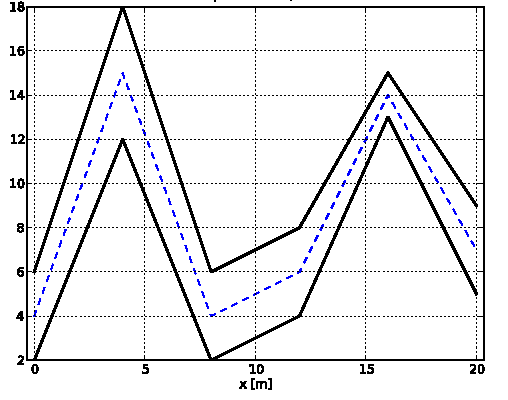
\includegraphics{figures/slalom_pic.pdf} 
%[width=.45\textwidth,height=.25\textheight,angle=0]
\end{center}
\caption{\label{fig:slalom_pic.pdf}  Slalom problem with $n=6$ gates. The initial and final positions are fixed and not included in the figure. The skier slides from left to right. The middle path is dashed and connects the center points of gates.}
\end{figure}

\begin{table}[h]
\caption{Problem data for Problem 2.}
\begin{center}
\[
\begin{array}{c|ccc}
i & x_i & y_i & c_i \\\hline
0 & 0 & 4 & N/A \\
1 & 4 & 5 & 3 \\
2 & 8 & 4 & 2 \\
3 & 12 & 6 & 2 \\
4 & 16 & 5 & 1 \\
5 & 20 & 7 & 2 \\
6 & 24 & 4 & N/A
\end{array}
\]
\end{center}
\label{tab:qplp-data-slalom}
\end{table}
\begin{enumerate}
\item {[Optimization Problem Expression]} Given the data $\{(x_i, y_i, c_i)\}_{i=0}^{n+1}$, write an optimization problem that minimizes the total length of the path. Your answer should come in the form of an SOCP. 
\newline
\newline
\newline
\newline
\sol{\item $g(x_1,x_2) = \dfrac{x_1^2}{4} + \dfrac{x_2^2}{9}$


}
\newline
\item Solve the problem numerically with the data given in Table~\ref{tab:qplp-data-slalom}.
\newline
\sol{\item Show that the following inequalities hold for any vector $x \in \Real{n}$:
\[
% \|x\|_\infty \le \|x\|_1 \le n \|x\|_\infty \\
% \|x\|_2 \le \|x\|_1 \le \sqrt{n} \|x\|_2 \\
% \|x\|_\infty \le \|x\|_2 \le\sqrt{n}\|x\|_\infty \\
\frac{1}{\sqrt{n}}\|x\|_2 \leq \|x\|_\infty \leq  \|x\|_2 \leq \|x\|_1 \leq \sqrt{n} \|x\|_2 \le n\|x\|_\infty.
\]

\textit{Hint:} For $\|x\|_1\leq \sqrt{n}\|x\|_2$, how might you express $\|x\|_1$ as the dot product of two vectors? Can you then use the Cauchy-Schwarz inequality to bound this dot product?}
\newline
\end{enumerate}
\newpage
\qns{Sphere enclosure}

{[Few lines of justification]} Let $B_i$, $i=1,\ldots,m$, be $m$ Euclidean balls in $\Real{n}$, with centers $x_i$, and radii
$\rho_i\geq 0$. We wish to find a ball $B$ of minimum radius that contains all the $B_i$, $i=1,\ldots,m$.
Cast this problem as an SOCP.

\sol{\item $g(x_1,x_2) = \dfrac{x_1^2}{4} + \dfrac{x_2^2}{9}$


}

\end{qunlist}
\end{document}
